\section{Introduction}\label{sec:intro}
% The success of reinforcement learning (RL) in competitive game playing has led to significant efforts to design better algorithms, collect more data, and build larger policy models. 
% ~\citep{badia2020agent57} and against humans~\citep{silver2016alphago,berner2019dota}, 
% has led to research on using RL models for human-centered applications such as healthcare~\citep{yu2019rlhealth}, economics~\citep{trott2021aieconomist} and robotics~\citep{kober2013robotics}. A large focus of the current literature has been on designing data-efficient algorithms, collecting larger amounts of data, and scaling up policy models. However, designing more efficient algorithms is not enough: RL algorithms for a human-centered applications must also be safe and aligned with human objectives~\citep{bommansani2021foundational}. %additional emphasis on these human-centred applications differ fundamentally from traditional RL applications along a different axis  -- these necessitate that RL models are safe and aligned with human objectives.

% %In order to do so, one has to be careful in specifying the reward functions which the RL model is optimized over; slight misspecifications here can lead to unintended, potentially catastrophic behaviors~\citep{hadfield2017ird}.  %Specifying such accurate reward functions is challenging for humans, leading agents to optimize misspecified rewards. %HRumans typically struggle to design accurate reward functionsDesigning such accurate reward functions can be very challenging for humans, leading to agents optimized on misspecified rewards.  
% There is already some evidence that safety constraints may be a bottleneck. Indeed, \emph{reward hacking}, or the gaming of misspecified proxy reward functions by RL agents, has appeared in a variety of contexts, such as game playing~\citep{clark2016faultyreward,ibarz2018humandemo}, robotics~\citep{popov2017dexterous, christiano2017preflearning}, text summarization~\citep{paulus2018drl_summarization}), and autonomous driving~\citep{knox2021misdesign}. In a boat racing game, when asked to maximize the score as a proxy for finishing first in the race, an agent instead learned to circle between two checkpoints to collect points~\citep{clark2016faultyreward}.

As reinforcement learning agents are trained with better algorithms, more data, and larger policy models, they are at increased risk of overfitting their objectives \citep{russell2019human}. \emph{Reward hacking}, or the gaming of misspecified reward functions by RL agents, has appeared in a variety of contexts, such as game playing~\citep{ibarz2018humandemo}, 
%clark2016faultyreward, robotics~\citep{popov2017dexterous, christiano2017preflearning}, 
text summarization~\citep{paulus2018drl_summarization}, and autonomous driving~\citep{knox2021misdesign}. %We list more examples in Section~\ref{sec:related}.
These examples show that better algorithms and models are not enough; for human-centered applications such as healthcare~\citep{yu2019rlhealth}, economics~\citep{trott2021aieconomist} and  robotics~\citep{kober2013robotics}, RL algorithms must be safe and aligned with human objectives~\citep{bommansani2021foundational,hubinger2019risks}. 

Reward misspecifications occur because real-world tasks have numerous, often conflicting desiderata. In practice, reward designers resort to optimizing a proxy reward that is either more readily measured or more easily optimized than the true reward. For example, %consider the task of placing a red block on top of a blue block~\citep{popov2017dexterous}. Instead of optimizing for the intended behavior, which has a sparse reward (only one state has nonzero reward), it is easier optimize for a proxy, such as maximizing the height of the red block, which is a more continuous signal. As another example, 
consider a recommender system optimizing for users' subjective well-being (SWB). Because SWB is difficult to measure, engineers rely on more tangible metrics such as click-through rates or watch-time. Optimizing for misspecified proxies led YouTube to overemphasize watch-time and harm user satisfaction~\citep{stray2020recommendersystem}, as well as to recommended extreme political content to users~\citep{times2019brazil}. %We expand on the different types of misspecifications that can arise in Section~\ref{sec:misspec}.  %and is therefore challenging to directly optimize for. Therefore, a reward designer must rely on a denser proxy signal, such as the height of the red block. S, and design a reward function that optimizes such a signal. FinalOne common source of error is a conceptual misunderstanding of the behavior a reward function actually incentivizes.  This task has Even simple tasks, such as For example, formulating a function that correctly captures intended behavior is challenging. Even on simple tasks, such training a Why are reward functions often misspecified? Misspecified reward functions are not Reward functions are often misspecified because of limitations in Most RL algorithms require the designer to specify a reward function, which a policy optimizes for. However, formulating a function that correctly encompasses the desiderata of the underlying task is challenging. What is a reasonable reward that encourages stacking a red block on top of a blue block? When the agent is rewarded for increasing the height of the bottom of the red block, it instead learns to flip the red block over~\citep{popov2017dexterous}. Specifying rewards for more challenging tasks such as text summarization or autonomous driving is even more challenging. In practice, almost all rewards teach policies to approximate the intended behavior

Addressing reward hacking is a first step towards developing human-aligned RL agents and one goal of ML safety~\citep{Hendrycks2021UnsolvedPI}. However, there has been little systematic work investigating when or how it tends to occur, or how to detect it before it runs awry. To remedy this, we study the problem of reward hacking across four diverse environments: traffic control~\citep{wu2017flow}, COVID response~\citep{kompella2020pandemic}, blood glucose monitoring~\citep{fox2020bgp}, and the Atari game Riverraid~\citep{brockman2016gym}. Within these environments, we construct nine misspecified proxy reward functions (Section~\ref{sec:setup}).  %with errors such as incorrect scope or incorrect ontology.%We cover our design of these environments and rewards in Section~\ref{sec:realism}.

%These environments 
%, chosen to mirror real-world systems, are intended to 
%serve as a case study for mapping how reward misspecification might affect learned RL models in the future.  %is therefore an important problem in ML safety While such reward hacking behavior can pose problems for training human-aligned RL agents~\citep{Hendrycks2021UnsolvedPI}, there has been little systematic work investigating when or how it tends to occur, or how to detect it before it runs awry. To remedy this, we systematically study this problem of reward misspecification across a diverse set of four environments: traffic control~\citep{wu2017flow}, COVID response~\citep{kompella2020pandemic}, blood glucose monitoring~\citep{fox2020bgp}, and the Atari game Riverraid~\citep{brockman2016gym}. These environments, chosen to mirror real-world systems, are intended to serve as a case study for mapping how reward misspecification might affect the behavior of learnt RL models in the future. 

%To understand the question of how misspecifications arise, we create a conceptual taxonomy of reward misspecifications. Our taxonomy focuses on three scenarios of how the proxy reward may diverge from the true reward: 1) \emph{Misweighting}, where rewards differ in the relative importance they give to each sub-metric, 2) \emph{Ontological}, where the rewards differ in the grounding of the human objective, and 3) \emph{Scope}, which covers misspecification in the domain over which rewards are measured. This taxonomy is discussed in detail in Section~\ref{}. 

%o understand this taxonomy, consider trying to optimize for smooth traffic flow in a road network. This typically involves rewarding high velocities (less congestion, faster commutes) and penalizing high vehicle accelerations (more emissions, rougher driving).


%, modeled after how these arise in the real world. %comprises three different forms of misspecification, depending on how these arise in the real-world. 

\begin{figure}[tbp]
%\captionsetup[subfigure]{labelformat=empty}
%\captionsetup{format=plain, font=small}
\centering
\includegraphics[scale=0.21]{figures/graphics_gray/misspecification_gray_2.eps}%
% \hfill
% \subfloat[\label{fig:main_capabilities}] {\includesvg[scale=.58]{figures/graphics_gray/agent_capabilities_gray.svg}}%

% \subfloat[\label{fig:main_qualitiative}] {\includesvg[scale=0.14]{figures/graphics_gray/qual_policy_horizontal_gray.svg}}%

% \subfloat[\label{fig:main_mis}] {\includesvg[scale=0.2]{figures/graphics_gray/misspecification_gray.svg}}%
% \hfill
% \subfloat[\label{fig:main_capabilities}] {\includesvg[scale=.68]{figures/graphics_gray/agent_capabilities_gray.svg}}%

% \subfloat[\label{fig:main_qualitiative}] {\includesvg[scale=0.15]{figures/graphics_gray/qual_policy_gray.svg}}%
% \hfill
% \subfloat[\label{fig:main_detector}] {\includesvg[scale=0.16]{figures/graphics_gray/detector_gray.svg}}%
% \hfill

\caption{An example of reward hacking when cars merge onto a highway. A human-driver model controls the grey cars and an RL policy controls the red car. The RL agent observes positions and velocities of nearby cars (including itself) and adjusts its acceleration to maximize the proxy reward. At first glance, both the proxy reward and true reward appear to incentivize fast traffic flow. However, smaller policy models allow the red car to merge, whereas larger policy models exploit the misspecification by stopping the red car. When the red car stops merging, the mean velocity increases (merging slows down the more numerous grey cars). However, the mean commute time also increases (the red car is stuck). This exemplifies a \emph{phase transition}: the qualitative behavior of the agent shifts as the model size increases.}
\label{fig:main}
\end{figure}
%\vspace{-5mm}

Using our environments, we study how increasing optimization power affects reward hacking, by training RL agents with varying resources such as model size, training time, action space resolution, and observation space noise (Section~\ref{sec:measurement}). We find that more powerful agents often 
attain higher proxy reward but lower true reward, as illustrated in Figure~\ref{fig:main}. Since the trend in ML is to increase resources exponentially each year \citep{ai100report2021}, this suggests that reward hacking will become more pronounced in the future in the absence of countermeasures.

%Because these misspecifications are caused by resource limitations, they are fundamental constraint on our ability to optimize for our intended behavior. 
%With this taxonomy, we look at \emph{how reward misspecification becomes reward hacking} -- in other words, why misspecification can be problematic. As computational resources increase and algorithms improve, machine learning models have become stronger optimizers~\citep{kaplan2020scaling}. We study how increasing optimization power drives reward hacking. 
%Moving past previous work, we identify factors driving reward hacking, highlighting the need for greater study of this problem. 
%In particular, we test the hypothesis that more capable models tend to overfit their rewards more.

%We examine four notions of model capabilities: policy model size, optimization steps, action space resolution, and observation space noise. 

%For each of these, we study both qualitative trends, observing how policy behavior changes as a function of its capabilities, and quantitative trends, measuring the deviation between proxy and true rewards as we vary model capabilities. 

More worryingly, we observe several instances of \emph{phase transitions}. In a phase transition, the more capable model pursues a qualitatively different policy that sharply decreases the true reward. Figure~\ref{fig:main} illustrates one example: An RL agent regulating traffic learns to stop any cars from merging onto the highway in order to maintain a high average velocity of the cars on the straightaway. 

Since there is little prior warning of phase transitions, they pose a challenge to monitoring the safety of ML systems.
Spurred by this challenge, we propose an anomaly detection task~\citep{Hendrycks2017ABF, %Hendrycks2019DeepAD, 
Tack2020CSIND}: Can we detect when the true reward starts to drop, while maintaining a low false positive rate in benign cases? We instantiate our proposed task, \textsc{Polynomaly}, for the traffic and COVID environments (Section~\ref{sec:detection}). Given a trusted policy with moderate performance, one must detect whether a given policy is aberrant. %To evaluate performance on this task, we propose two metrics of measuring detection strength: \kbcomm{describe the metrics here}. 
We provide several baseline anomaly detectors for this task and release our data at \url{https://github.com/aypan17/reward-misspecification}. 




% %Because these misspecifications are caused by resource limitations, they are fundamental constraint on our ability to optimize for our intended behavior. 
% With this taxonomy, we look at \emph{how reward misspecification becomes reward hacking} -- in other words, why misspecification can be problematic. As computational resources increase and algorithms improve, machine learning models have become stronger optimizers~\citep{kaplan2020scaling}. We study how increasing optimization power drives reward hacking. 
% %Moving past previous work, we identify factors driving reward hacking, highlighting the need for greater study of this problem. 
% In particular, we test the hypothesis that more capable models tend to overfit their rewards more.

% We examine four notions of model capabilities: policy model size, optimization steps, action space resolution, and observation space noise. For each of these, we study both qualitative trends, observing how policy behavior changes as a function of its capabilities, and quantitative trends, measuring the deviation between proxy and true rewards as we vary model capabilities. 

% Figure~\ref{fig:main_capabilities} exhibits the key insight of our paper. We observe that more capable models, in general, attain higher proxy reward but lower true reward. We also observe several examples of \emph{phase transitions}. In a phase transition, the more capable model pursues a qualitatively different policy that often has unintended consequences. For example, as illustrated in Figure~\ref{fig:main_qualitative}, an RL agent regulating traffic learns to stop any cars from merging onto the highway in order to maintain a high average velocity of the cars on the straightaway. %We illustrate this qualitative shift in Figure~\ref{fig:main_qualitiative}. 
% Phase transitions are particularly problematic, because they could lead to sudden and unexpectedly worse performance.  % across the four different misspecifications mentioned above. 

% Motivated by phase transitions, we propose an anomaly detection task~\citep{Hendrycks2017ABF, Hendrycks2019DeepAD, Tack2020CSIND}: Can we detect when the true reward starts to drop, while maintaining a low false positive rate in benign cases? Our proposed task, which we instantiate for the traffic and COVID environments, is highlighted in Figure~\ref{fig:main_detector}. To evaluate performance on this task, we propose two metrics of measuring detection strength: \kbcomm{describe the metrics here}. Additionally, we provide several baseline anomaly detectors for this task and evaluate them on the proposed metrics. We release our data with the hope of spurring more research into detecting reward misspecification. 